\section{Introduction}

% % Requires: \usepackage{tikz}
% \usetikzlibrary{positioning, arrows.meta}

\begin{figure}[t]
\centering
\begin{tikzpicture}[
    root/.style={circle, draw=black!60, thick, minimum size=0.8cm, font=\normalsize},
    noised/.style={circle, draw=blue!70!black, thick, fill=blue!10, minimum size=0.8cm, font=\normalsize},
    derived/.style={rectangle, rounded corners=3pt, draw=gray!60, fill=gray!8, font=\normalsize, inner sep=5pt},
    tgt/.style={rectangle, rounded corners=3pt, draw=orange!60, fill=orange!6, font=\normalsize, inner sep=5pt},
    arr/.style={-{Stealth[length=5pt]}, thick},
    same/.style={draw=black!30, thick, dashed, rounded corners=2pt},
]

% === User agent label ===
\node[font=\small\bfseries, text=black!40, rotate=90, anchor=south] at (-2.2, -0.7) {User agent $\mathcal{U}$};

% === Row 1: Private roots ===
\node[root] (x1) at (0, 0) {$x_1$};
\node[root] (x2) at (2.0, 0) {$x_2$};
\node[root] (x3) at (4.0, 0) {$x_3$};
\node[font=\small, text=black!50, anchor=east] at (-0.7, 0) {private};

% === Row 2: Noised roots ===
\node[noised] (xh1) at (0, -1.5) {$\hat{x}_1$};
\node[noised] (xh2) at (2.0, -1.5) {$\hat{x}_2$};
\node[noised] (xh3) at (4.0, -1.5) {$\hat{x}_3$};
\node[font=\small, text=blue!60, anchor=east] at (-0.7, -1.5) {cached};

\draw[arr, blue!60, densely dashed] (x1) -- node[right, font=\scriptsize, text=blue!50] {$\mathcal{M}$} (xh1);
\draw[arr, blue!60, densely dashed] (x2) -- node[right, font=\scriptsize, text=blue!50] {$\mathcal{M}$} (xh2);
\draw[arr, blue!60, densely dashed] (x3) -- node[right, font=\scriptsize, text=blue!50] {$\mathcal{M}$} (xh3);

% === Divider ===
\draw[thick, black!20] (-1.5, -2.4) -- (5.0, -2.4);
\node[text=black!40, anchor=east] at (-1.6, -2.4) {post-processing};

% === Adversary label ===
\node[font=\small\bfseries, text=black!40, rotate=90, anchor=south] at (-2.2, -4.0) {Adversary $\mathcal{A}$};

% === Row 3: Adversary queries ===
\node[derived] (q1) at (-0.4, -3.4) {$\hat{x}_1$};
\node[derived] (q2) at (1.2, -3.4) {$\hat{x}_1$};
\node[derived] (q3) at (3.6, -3.4) {$f(\hat{x}_2, \hat{x}_3)$};

\node[font=\scriptsize, text=black!40] at (-0.7, -3.9) {turn 1};
\node[font=\scriptsize, text=black!40] at (1.2, -3.9) {turn 2};
\node[font=\scriptsize, text=black!40] at (3.9, -3.9) {turn 3};

% === "Same value" annotation ===
\draw[same] (-0.9, -3.1) rectangle (1.7, -3.7);
\node[font=\scriptsize, text=black!45, anchor=east] at (-0.5, -2.90) {same cached value};

% === Row 4: Target ===
\node[tgt] (qT) at (1.8, -5.0) {$T(\hat{x}_1, \hat{x}_2, \hat{x}_3)$};
\node[font=\scriptsize, text=black!40] at (0.0, -5.0) {turn 4};

% === Arrows from cached to queries ===
\draw[arr, black!30] (xh1) -- (q1);
\draw[arr, black!30] (xh1) -- (q2);
\draw[arr, black!30] (xh2) -- (q3);
\draw[arr, black!30] (xh3) -- (q3);

% === Arrows to target ===
\draw[arr, black!30] (q1.south) -- (qT.north west);
\draw[arr, black!30] (q3.south) -- (qT.north east);

\end{tikzpicture}
\caption{Overview of \sysname{}. The user agent sanitizes private roots once and caches them (blue). All adversary queries are answered from the cached roots (gray): repeated requests return the identical value (turns 1--2), derived computations are deterministic (turn 3), and the target incurs no additional privacy cost (turn 4).}
\label{fig:dag_overview}
\end{figure}
\begin{figure*}
    \centering
    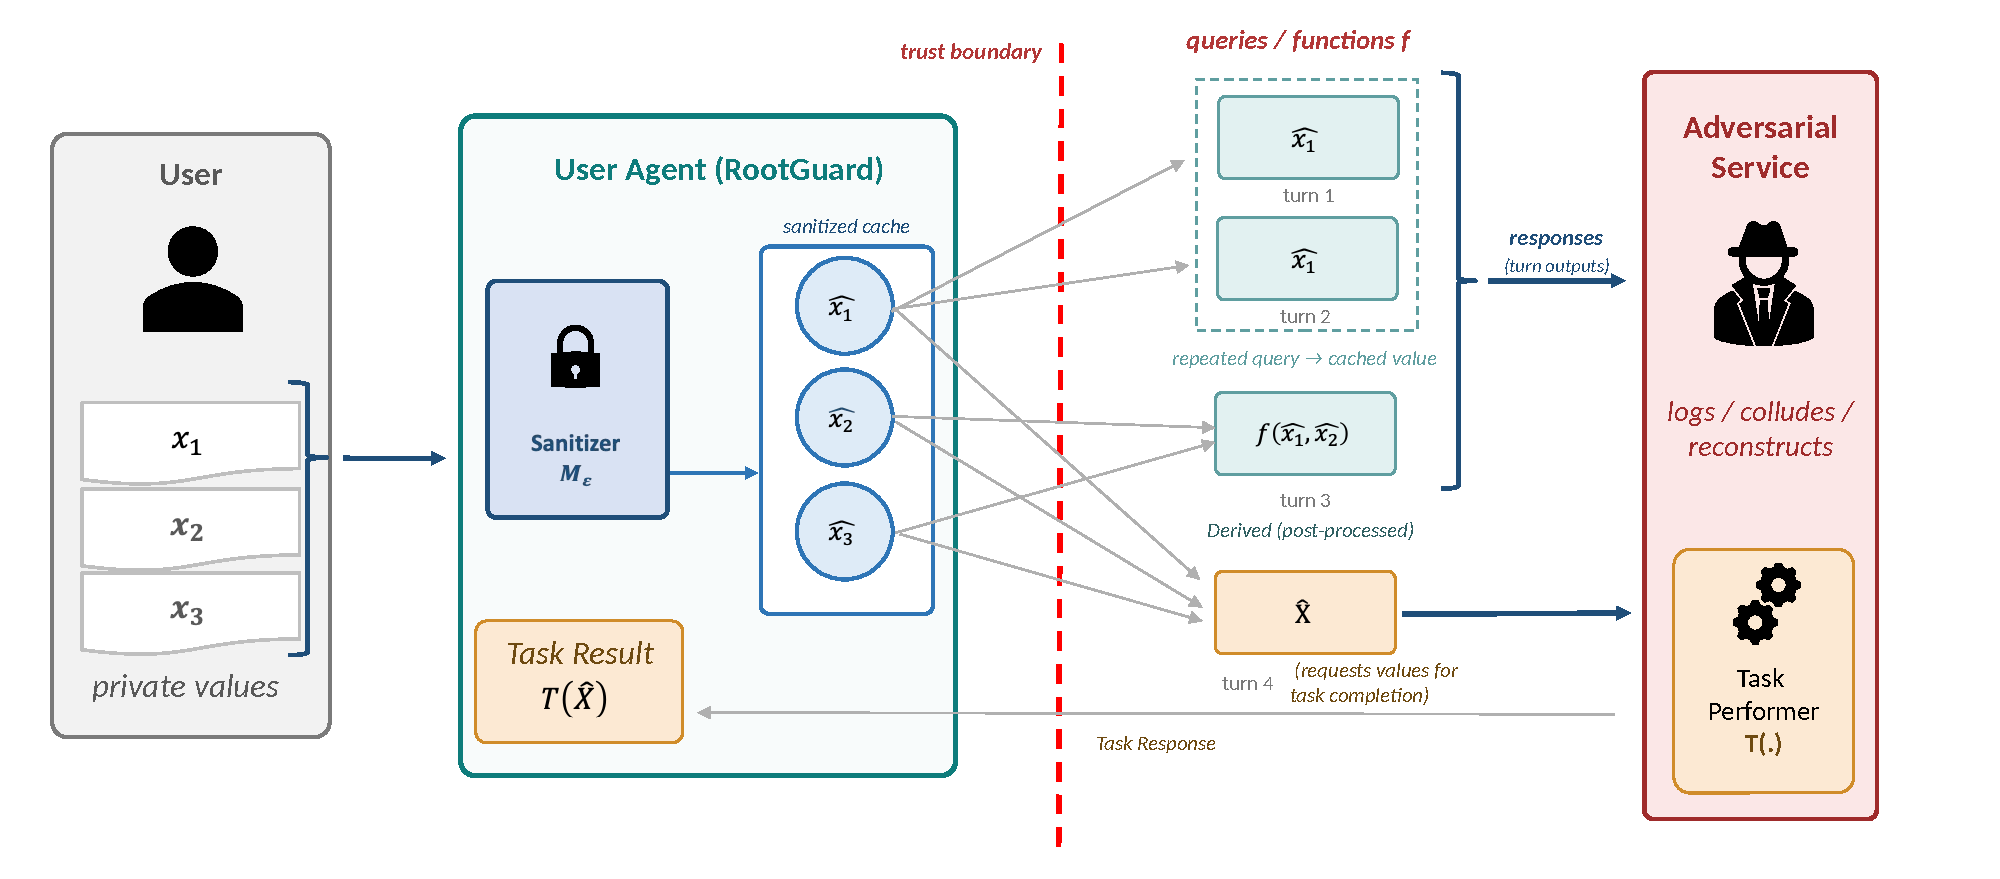
\includegraphics[width=0.8\linewidth]{figures/rootguard_overview.pdf}
    \caption{Overview of \sysname{} in an agentic deployment. At initialization, the user passes its private values $X = (x_1, x_2, x_3)$ to the user agent, which sanitizes each root once via $\mathcal{M}_\varepsilon$ and stores the result in the sanitized cache. All subsequent interactions with the adversarial service are answered from the cache: repeated requests for the same root return the identical cached value (turns 1, 2), derived requests are deterministic post-processing of cached roots (turn 3), and the request that supplies all roots for task computation (turn 4) carries no additional privacy cost. The trust boundary separates the user agent from the adversarial service, which performs the user's task by computing $T(\hat{X})$ and may concurrently log, collude with other parties, or attempt to reconstruct the underlying $X$. The task result $T(\hat{X})$ is returned to the user agent. By the post-processing theorem, the adversary's view across the boundary is no more informative than the initial root sanitization, regardless of which functions $f$ it requests.}
\label{fig:rootguard_overview}
\end{figure*}

The rapid integration of large language models into sensitive domains, such as healthcare, finance, legal consultation, etc. has created a new attack surface for privacy. Users are increasingly delegating tasks to LLM agents that act on their behalf, accessing external tools and services via protocols such as  MCP~\cite{anthropic2024mcp,hou2025mcp}, and executing multi-step workflows. For instance, a medical agent might submit lab values to a diagnostic service, forward results to a medication advisor, and send recommendations to insurance providers, all without human oversight of the private data released at each step.

Every intermediary in this chain is a potential adversary. Services can be malicious by design, collecting private data under the guise of providing a task. They can be compromised through prompt injection attacks~\cite{greshake2023indirect,zhan2024injecagent,debenedetti2024agentdojo}, where adversarial inputs force an agent to reveal user data or compute unintended functions on sensitive information, or they can be coerced through legal processes~\cite{openai-nyt} or breached through conventional exploits. Therefore, client-side privacy protection is not only a precaution against dishonest providers, it is a necessary defense against the compromise of honest ones. The user agent must therefore assume that \emph{any} value released to \emph{any} service may be exposed, and sanitize accordingly.

The standard defense is to add noise to each released value independently, using metric differential privacy~\cite{Chatzikokolakis2013BroadeningTS}. Methods such as Pr$\epsilon\epsilon$mpt~\cite{chowdhury2025} and CAPE~\cite{wu2025capecontextawarepromptperturbation} protect individual tokens in a prompt with formal guarantees. However, these methods treat each release in isolation, disregarding the relationships between released values. This independence assumption breaks down in practice --- even when all parties are honest.

% \paragraph{Benign leakage.}
% Consider two routine scenarios that arise naturally in agentic workflows:
 
% \begin{itemize}
%     \item \textbf{Cross-platform redundancy.} A user's agent shares the same lab value, say, fasting glucose, with a diabetes screening service and a metabolic health dashboard. Each service receives an independently noised copy. If either service is later breached or subpoenaed, the attacker holds two independent views of the same value. By the composition theorem~\cite{dwork2006calibrating}, the joint privacy cost is $2\varepsilon$, not $\varepsilon$. As agents interact with more services, the effective privacy budget scales linearly with the number of releases.
 
%     \item \textbf{Structural redundancy.} A user releases both a private root value and a derived value that depends on it --- for example, height and BMI. Each release is independently noised. But the adversary now holds two independent views of the same underlying root (i.e., height). We show (Theorem~\ref{thm:privacy-leakage}) that the effective distinguishability of the root is amplified by up to the Lipschitz constant of the deriving function --- for nonlinear functions common in medical and financial domains (ratios, reciprocals, logarithms), this amplification can exceed $100\times$ the nominal privacy parameter. 
%     % \sarthak{This could be too much detail, maybe say we formalize the leakage of privacy from this structure in Theorem in terms of the dependencies ....}
% \end{itemize}

\paragraph{Benign leakage.} Two routine scenarios suffice to break the per-release guarantee. \emph{Cross-platform redundancy:} a single root (e.g., fasting glucose) sent to two services arrives as two independently noised copies, costing $2\varepsilon$ rather than $\varepsilon$ by composition~\cite{dwork2006calibrating}; the budget scales linearly with services touched. \emph{Structural redundancy:} a root and a derived value (e.g., height and BMI) released separately each leak the root, and we show (Theorem~\ref{thm:privacy-leakage}) that for nonlinear derivations the effective distinguishability is amplified by the Lipschitz constant --- exceeding $100\times$ the nominal $\varepsilon$ for common medical formulas.

\noindent These are natural consequences of how independently-noising methods interact with multi-service, multi-value workflows. 

\paragraph{Adversarial leakage.} The problem is severe in adversarial settings. Services can be compromised through prompt injection~\cite{greshake2023indirect,zhan2024injecagent,debenedetti2024agentdojo}, giving the adversary control of the interaction. It can then request the same value repeatedly (averaging away protection at rate $1/\sqrt{q}$), force computation of arbitrary derived functions (each a fresh independent observation), or exploit the target release as a cross-root constraint linking all private values through the task function.


% \paragraph{Adversarial leakage.}
% The problem is severe in adversarial settings. Services can be compromised through prompt injection attacks~\cite{greshake2023indirect,zhan2024injecagent,debenedetti2024agentdojo}, where adversarial inputs force an agent to reveal user data or compute unintended functions on sensitive information. In the worst case, the adversary controls the interaction and can:
 
% \begin{itemize}
%     \item request the same private value \emph{repeatedly}, obtaining $q$ independent noise draws and averaging away the privacy protection (reconstruction error decreases as $1/\sqrt{q}$);
%     \item force the agent to compute \emph{arbitrary functions} of private data, each producing a fresh, independently noised observation that can be combined with previous releases;
%     \item exploit the \emph{target release} itself as a cross-root constraint, linking all private values through the known task function.
% \end{itemize}

\paragraph{The fundamental problem.} Both the benign and adversarial scenarios are instances of the same root cause: \emph{uncontrolled independent releases} of correlated private values. Without a mechanism to track dependencies between releases, every additional interaction, whether benign or adversarial, degrades the user's privacy beyond the nominal budget. Existing sanitizers~\cite{chowdhury2025,wu2025capecontextawarepromptperturbation} are stateless: they treat each value in isolation, discarding structural information that is already present in the interaction protocol.
 
\paragraph{Our approach.} We propose \sysname{}, a dependency-aware privacy mechanism for multi-turn agentic interactions. We noise the private root values exactly once, and compute everything else deterministically from the noised roots. By the post-processing theorem of differential privacy~\cite{dwork2014algorithmic}, all derived values, regardless of the function the adversary chooses, inherit privacy at zero additional cost. Repeated queries return the same cached value. Cross-platform releases of the same root are identical. The adversary's view after $t$ turns is no more informative than after the first release.

This creates a \emph{double asymmetry}. When the adversary forces $t$ turns of interaction, the total privacy budget $B = t\varepsilon$ scales with $t$; \sysname{} redistributes this larger budget across the $k$ roots, while independent noising spends $\varepsilon$ per release. As a result, with additional turns, \sysname{}'s utility improves (more budget per root) while its privacy stays constant (all releases are post-processing). Independent noising gains nothing, since the target is always a single release at $\varepsilon$, but its privacy degrades with each fresh independent observation.
 
% \paragraph{Exploiting domain knowledge.} 
% \divyam{Simplify this!}
% Crucially, the structural knowledge needed to eliminate these failures is increasingly available. In the agentic setting, service protocols such as MCP require providers to publish tool schemas~\cite{anthropic2024mcp}, such as parameter names, types, and descriptions of the computations they perform. A medical service that exposes a tool \texttt{computeBMI(height, weight)} explicitly declares a functional dependency. Beyond protocol metadata, many derived values rely on standardized, public formulas (e.g., BMI, eGFR, HOMA-IR, FIB-4) that a domain-aware agent can recognize without any service cooperation.
 
% \sysname{} exploits this knowledge at three progressive levels:
% \begin{enumerate}
%     \item \textbf{Root identification} (Level 1): knowing which values are independent roots eliminates redundant noising of derived values and concentrates the budget on roots.
%     \item \textbf{Inter-root dependencies} (Level 2): identifying dependencies between roots allows privacy to be inherited for free (Theorem~\ref{thm:implied-privacy}), freeing budget for truly independent roots.
%     \item \textbf{Target sensitivity} (Level 3): \divyam{specify that even an approximate $\hat{f}$ helps; any indication of target sensitivity is better than nothing} knowing the target function enables sensitivity-weighted budget allocation, $\varepsilon_i \propto (|h_i| \cdot D_i)^{1/2}$, which minimizes target error by directing budget to the roots that matter most (Sec.~\ref{sec:opt-budget}).
% \end{enumerate}
 
% \noindent Each level requires only public information (tool schemas, published formulas, population statistics) and improves the privacy-utility tradeoff without weakening the privacy guarantee.


\paragraph{Exploiting domain knowledge.} 
\sysname{} requires the user agent to identify sensitive values (the \emph{roots}) --- a baseline assumption shared with prior sanitizers~\cite{chowdhury2025,wu2025capecontextawarepromptperturbation}, typically discharged via NER or explicit user declaration. Beyond this, \sysname{} can exploit two progressive levels of public domain knowledge to improve the privacy-utility tradeoff. The structural knowledge needed is increasingly available: MCP tool schemas~\cite{anthropic2024mcp} declare parameter types and computations (e.g., \texttt{computeBMI(height, weight)}), and many derived values rely on standardized public formulas (BMI, eGFR, HOMA-IR, FIB-4) that a domain-aware agent can recognize without service cooperation.
 
\begin{enumerate}
    \item \textbf{Inter-root dependencies} (Level 1): identifying which declared roots are deterministic functions of others (e.g., BMI from height and weight) lets dependent values inherit privacy from their parents at zero cost (Theorem~\ref{thm:implied-privacy}), freeing budget for truly independent roots.
    \item \textbf{Target sensitivity} (Level 2): any indication of the target function's form --- whether the exact published formula or an approximation $\hat{f}$ --- enables sensitivity-weighted budget allocation, $\varepsilon_i \propto (|h_i| \cdot D_i)^{1/2}$, which minimizes target error by directing budget to the roots that matter most (Sec.~\ref{sec:opt-budget}).
\end{enumerate}
 
\noindent Each level requires only public information (tool schemas, published formulas, population statistics) and improves the privacy-utility tradeoff without weakening the privacy guarantee.
 
% \paragraph{Contributions.}
% \begin{itemize}
%     \item We formalize the multi-turn adversarial setting for agentic privacy and show that \sysname{}'s privacy guarantee depends only on the root sanitization parameters --- regardless of the adversary's function choices, query count, or interaction length (Theorem~\ref{thm:privacy-guarantee}).
%     \item We prove that independently noising a derived value amplifies the distinguishability of its parent root by the function's Lipschitz constant (Theorem~\ref{thm:privacy-leakage}), and that derived values computed from noised roots inherit privacy at zero marginal cost (Theorem~\ref{thm:implied-privacy}).
%     \item We demonstrate a double asymmetry on 8 medical diagnostic templates: at $\varepsilon = 0.1$, \sysname{} achieves $2.6\times$ lower target error than independent noising (7.8\% vs.\ 20.3\% wMAPE at $B = (2k{+}1)\varepsilon$), widening to $3.8\times$ at $(3k{+}1)\varepsilon$.
%     \item We show that independent noising is vulnerable to MAP reconstruction attacks that scale with query count: at matched per-root noise ($\varepsilon_r = 0.1$), the adversary's reconstruction wMAPE drops from 21.8\% to 6.2\% as $q$ (queries) increases from 1 to 16 --- a $3.5\times$ reduction in adversary error. \sysname{} is invariant: reconstruction wMAPE is identical at every $q$.
%     \item We confirm transfer to a real LLM-driven tool-call deployment: across 21{,}600 sessions in a GPT-5.4 nano agent harness, RQ1's privacy-utility ordering and per-template structure reproduce within bootstrap noise (Sec.~\ref{sec:experiments-rq4}).
% \end{itemize}
\paragraph{Contributions.}
\begin{itemize}
    \item We formalize multi-turn agentic privacy and prove \sysname{}'s guarantee depends only on root sanitization parameters, independent of adversary function choices or query count (Thm.~\ref{thm:privacy-guarantee}).
    \item We prove independently noising a derived value amplifies parent-root distinguishability by the function's Lipschitz constant (Thm.~\ref{thm:privacy-leakage}); derived values from noised roots inherit privacy at zero marginal cost (Thm.~\ref{thm:implied-privacy}).
    \item On 8 medical templates: \sysname{} achieves $2.6\times$ lower target wMAPE than independent noising at $\varepsilon = 0.1$, $B = (2k{+}1)\varepsilon$ ($7.8\%$ vs.\ $20.3\%$), widening to $3.8\times$ at $(3k{+}1)\varepsilon$.
    \item Under matched per-root noise ($\varepsilon_r = 0.1$), MAP reconstruction degrades $\mathcal{M}$-All from $21.8\%$ to $6.2\%$ wMAPE as queries grow $1{\to}16$ ($3.5\times$); \sysname{} is invariant.
    \item These findings transfer end-to-end: $21{,}600$ LLM tool-call sessions (GPT-5.4 nano) reproduce RQ1's ordering and per-template structure within bootstrap noise (Sec.~\ref{sec:experiments-rq4}).
\end{itemize}